\chapter{Lur'e Problem}
\section{Definition of the Lur'e problem and staibility}
\begin{figure}[H]
	\centering
	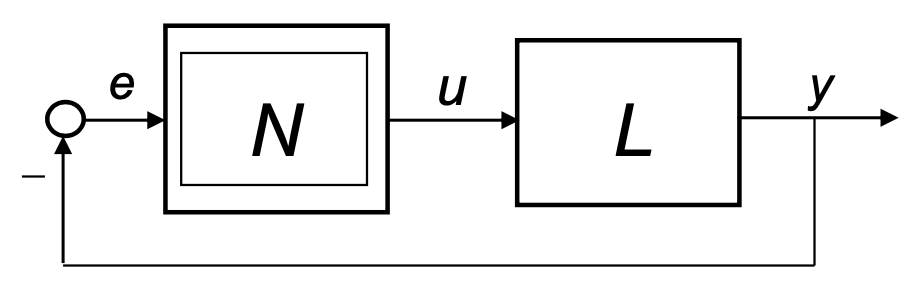
\includegraphics[scale=0.4]{immagini/lure1}
	\caption{Lur'e system}
	\label{fig:lure1}
\end{figure}
An autonomous Lur'e system is a feedback system with a nonlinear static component (N) in series with a linear component (L). The non linear part is defined with a function $\phi$ as follows: 
\[
N \colon u(t)=\phi(e(t)), \forall e 
\]with:
\begin{itemize}
		\item $\phi \colon \Re \to \Re$
		\item $\phi(\cdot) \in \Phi_{\left[k_1,k_2\right]}$.
\end{itemize}
While the linear part is simply:
\[
L:  \begin{cases}
	\dot{x}=Ax+Bu \\ y=Cx
\end{cases}
\] with the assumption of (A,B) reachable and (A,C) observable.
\\ The $\phi$ function is meant to be continuous and to belong to a \textbf{sector nonlinearity}.
\begin{figure}[H]
	\centering
	\includegraphics[scale=0.4]{immagini/snl}
	\caption{Sector nonlinearity}
	\label{fig:snl}
\end{figure}
The sector is plotted in the e-u space taking e as an input and u as the output and it's defined by two lines of slope $k_1$and $k_2$. The sector of nonlinearity is the sector that contains all the $\phi$ funcitons which satisfy the following condition:
\[
\Phi_{\left[k_1,k_2\right]}=\left\{\phi(\cdot)\colon (k_2e-u)(u-k_1e)\ge 0, u=\phi(e), \forall e \in \Re\right\}
\]
Since the sector enforce the function to pass from 0 in any case and: $f(x)\colon=Ax+B\phi(-Cx)$ if $\phi(0)\to 0$ also $f(0)\to 0$ and so $\bar{x}=0$ is an equilibrium for S, for any section nonlinearity $\phi(\cdot) \in \Phi_{\left[k_1,k_2\right]}$.
\subsubsection{Absolute stability in the sector $[k_1,k_2]$}
\begin{defn}
	System \textcolor{red}{S} is \textcolor{red}{absolutely stable in the sector $[k_1,k_2]$} if x=0 is a globally asymptotically stable (GAS equilibrium, for every sector non linearity) $\phi(\cdot) \in \Phi_{\left[k_1,k_2\right]}$.
\end{defn}
So the Lur'e problem, given the transfer function G(s) of the linear system L, \textcolor{red}{determine necessary and/or sufficient conditions for the absolute stability} of S in the sector $[k_1,k_2]$.
\subsection{Necessary condition for absolute stability} \label{S_L}
\begin{figure}[H]
	\centering
	\includegraphics[scale=0.4]{immagini/snl2}
	\caption{$\phi(\cdot) \in \Phi_{[k_1,k_2]}$}
	\label{fig:snl2}
\end{figure}
Since $\phi$ is a general static function in a sector, among all the nonlinear set of functions we have for sure also the linear ones, so if we want to get absolute stability in the sector we have to consider all the possible functions, including the linear ones. It's \textbf{necessary} that when we restrict the set of funcitons to the linear ones to have asymptotical stability, but it's not sufficient.
\begin{figure}[H]
	\centering
	\includegraphics[scale=0.4]{immagini/sl}
	\caption{$\phi(e)= ke  \in \Phi_{[k_1,k_2]}$}
	\label{fig:sl}
\end{figure}
If S is absolutely stable in $[k_1,k_2]$, then , $S_L$ is (globally) asymptotically stable for any $k \in [k_1,k_2]$. If $0 \in [k_1,k_2]$, then, system L with transfer function G(s) is asymptotically stable.\\
So if we have a \underline{given k}, system $S_L$ is asymptotically stable if and only if the Nyquist plot of G(s) encircles (anti-clockwise) the point in the complex plan corresponding to the real number $-\frac{1}{k}$ as many times as the number of poles of G(s) with positive real part (\emph{Nyquist criterion})
\begin{figure}[H]
	\centering
	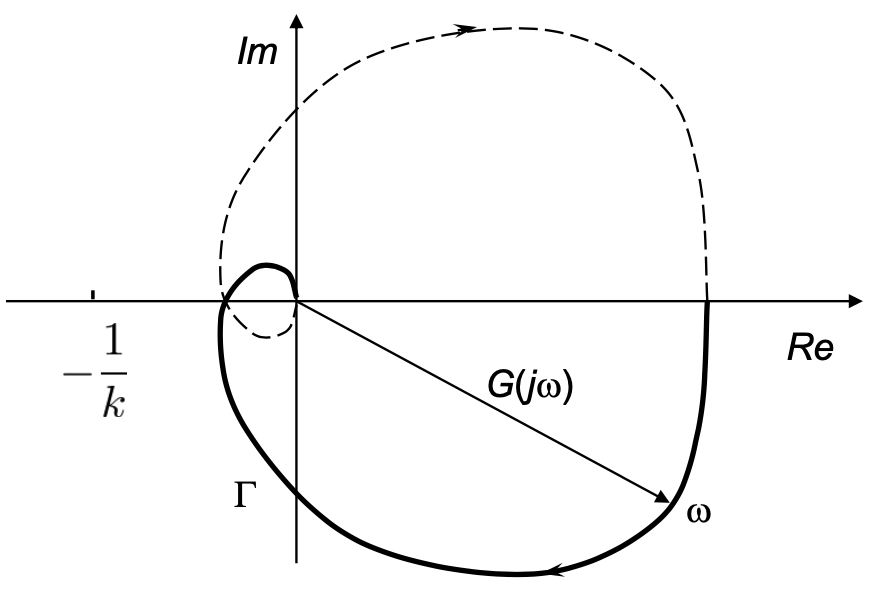
\includegraphics[scale=0.4]{immagini/nyq}
	\caption{Nyquist criterion}
	\label{fig:nyq}
\end{figure}
Now let's move a step further. Actually "k" can ranging in the sector $[k_1,k_2]$ so we can adapt the previous statement changing the value $-\frac{1}{k}$ with an interval defined as follows: \[I(k_1,k_2)\colon= \left\{\alpha \in \Re\colon \alpha =-\frac{1}{k}, k \in [k_1,k_2]\right\}\]
\begin{figure}[H]
	\centering
	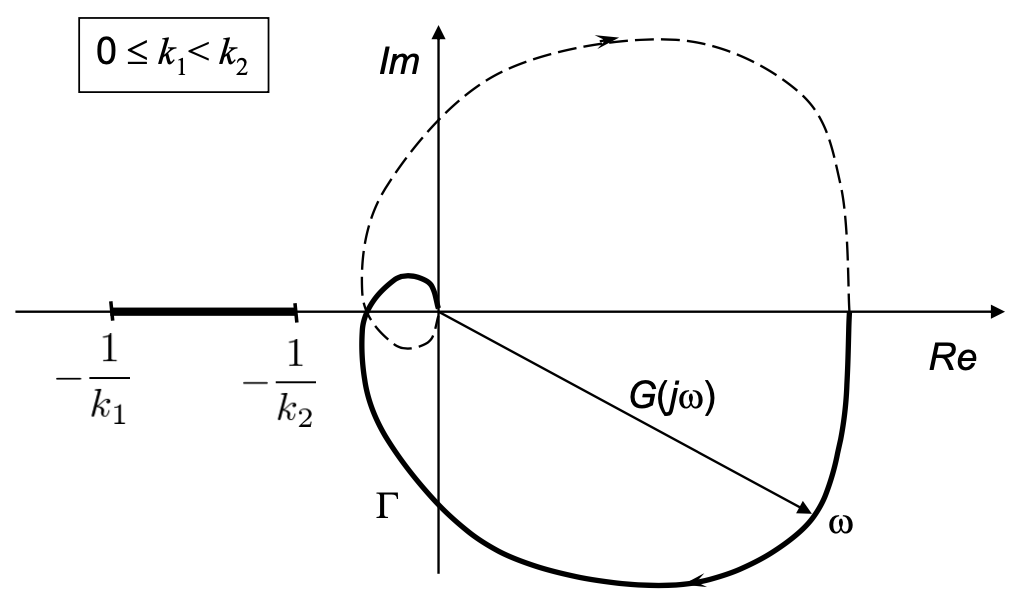
\includegraphics[scale=0.4]{immagini/nyq2}
	\caption{Nyquist criterion with an interval}
	\label{fig:nyq2}
\end{figure}
So for an \underline{uncertain k}, system $S_L$ is asymptotically stable for any $k\in[k_1, k_2]$ if and only if the Nyquist plot of G(s) encircles (anti-clockwise) $I(k_1,k_2)$ as many times as the number of poles of G(s) with positive real part.
\\ We can now state the theorem:
\begin{thm}[Necessary condition for absolute stability of an autonomous Lur'e system]
	If S is absolutely stable in the sector $[k_1, k_2]$, then the Nyquist plot of G(s) encircles (anti-clockwise) $I(k_1,k_2)$ as many times as the number of poles of G(s) with positive real part.
	In particular, if $0\in[k_1, k_2]$, then system L with transfer function G(s) is asymptotically stable.
\end{thm}
To sum up in Figure \ref{fig:nyqtot} are represented all the possible cases of sector configurations.
\begin{figure}[H]
	\centering
	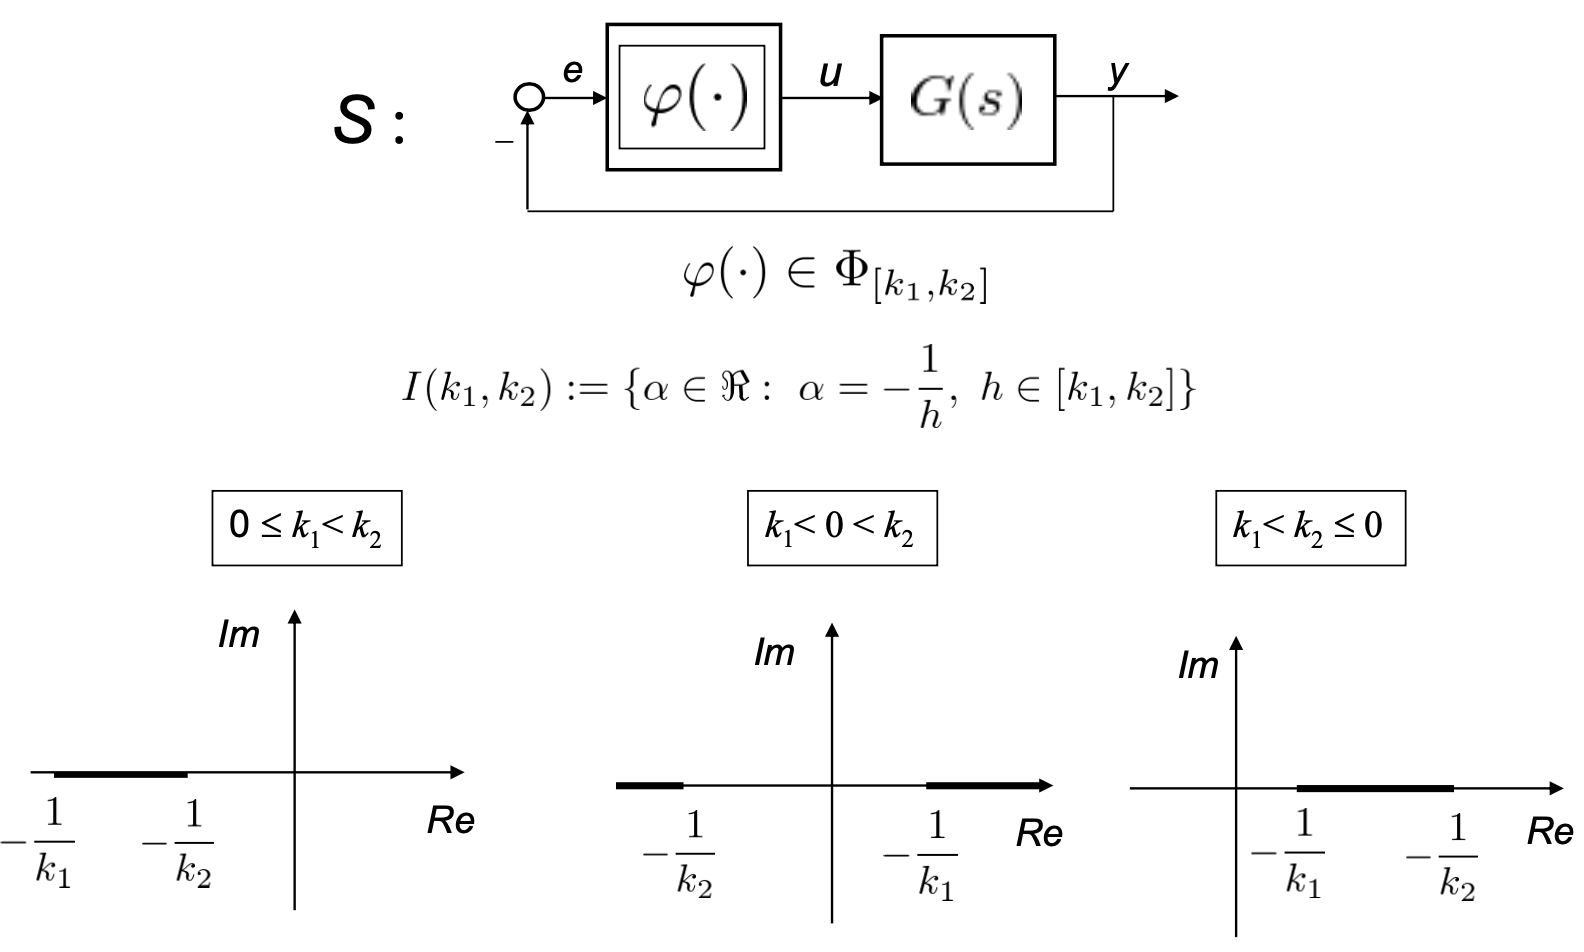
\includegraphics[scale=0.4]{immagini/nyqtot}
	\caption{Impact of the sector boundaries on Nyquist plot}
	\label{fig:nyqtot}
\end{figure}
 Notice that if one of the two ''k''s is equal to 0, one boundary of the interval \emph{I} diverges to infinity and so the Nyquist plot with the interval result as in Figure \ref{fig:nyq0}. So in practice in this case the Nyquist plot should not cross the semi line in question.
\begin{figure}[H]
 	\centering
 	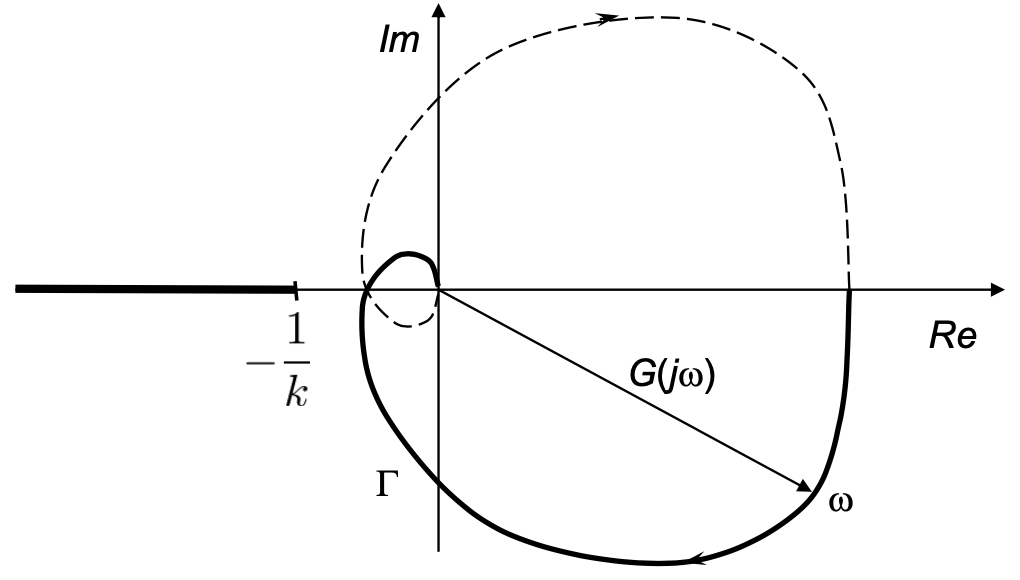
\includegraphics[scale=0.4]{immagini/nyq0}
 	\caption{$[0,k]$ sector}
 	\label{fig:nyq0}
\end{figure}
\subsection{Conjectures}
\subsubsection{Aizerman conjecture (1949):}
The necessary condition is also sufficient.
\subsubsection{Kalman conjecture (1960):}
If $\phi(\cdot)$ is differentiable with continuous derivative and it holds that 
\[
k_1\le\frac{d\phi}{de}(e)\le k_2, \qquad \forall e\in\Re
\]then the necessary condition is also sufficient.\\
But this conjectures are proven to be false with some non-trivial counterexamples we will omit. The fundamental message here is that the solution to Lur'e problem cannot be rephrased in terms of linear system analysis.
\linebreak
So now we want to study some sufficient and practical condition but not sufficient: the Popov and circle criteria.
\section{Popov Criterion}
\begin{thm}[sufficient condition for the absolute stability of S in sector \textcolor{red}{[0,k]}, Popov criterion, 1962] 
	System S is absolutely stable in sector [0,k] if system L is asymptotically stable (necessary condition), and if there exists a real number ''q'' such that the following condition is satisfied: 
	\[
	\Re\left[(1+j\omega q)G(j\omega\right)] > -\frac{1}{k}, \forall \omega \ge 0
	\]
\end{thm}
In order to better understand and use this theorem is very useful to have a sight at its graphical interpretation. 
\subsection{Graphical interpretation of Popov criterion}
We will work with a given transfer function G(s).\\  The first step is to draw the polar plot of G(s) setting \boxed{q=0} and check if it is entirely located on the right-hand-side of the straight line passing through $-\frac{1}{k}$ and parallel to the imaginary axis. In this way the necessary condition for absolute stability is satisfied.
\begin{figure}[H]
	\centering
	\includegraphics[scale=0.3]{immagini/popovq0} \qquad
	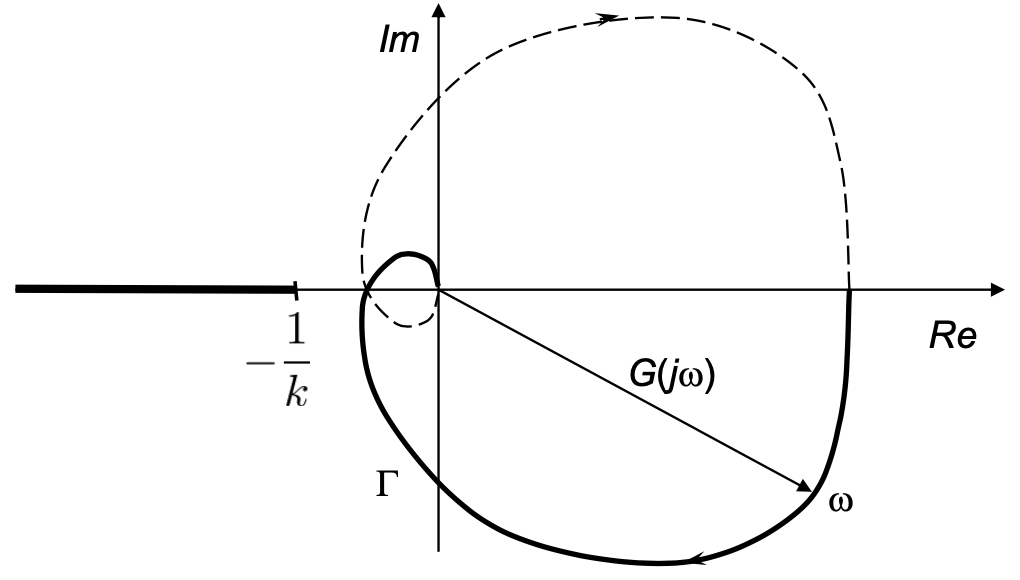
\includegraphics[scale=0.3]{immagini/nyq0}
	\label{fig:popovq0}
\end{figure}
Let's now remove the assumption of having q=0 and draw the polar plot $\Gamma^*$ of G*(s) with a \boxed{q\ne0}. We call this the Popov plot and essentially is a rescaled polar plot along the imaginary axis by $\omega$. For this reason the Popov plot and the polar plot shares the same points on the real axis.
\[
G^*(j\omega)=\operatorname{Re}[G(j\omega)]+j\omega\operatorname{Im}[G(j\omega)]
\]
\begin{figure}[H]
	\centering
	\includegraphics[scale=0.4]{immagini/popovplot}
	\caption{Popov plot}
	\label{fig:popovplot}
\end{figure}
We now have to find out if there exist a straight line passing through $-\frac{1}{k}$ (\emph{Popov line}) such that $\Gamma^*$ is on the open half plane on its right-hand-side. But how can we identify that line? Let's do a bit of computation.
\[
G^*(j\omega)=\operatorname{Re}[G(j\omega)]+j\omega\operatorname{Im}[G(j\omega)]
\]
\[ \operatorname{Re}[(1+j\omega q)G(j\omega)]=\operatorname{Re}[G(j\omega)]-q\operatorname{Im}[G(j\omega)]=a^*-qb^*\] where $a^*\colon=\operatorname{Re}[G^*(j\omega)]$ and $b^*\colon=\operatorname{Im}[G^*(j\omega)]$.
So applying the Popov criterion condition: \[\operatorname{Re}[(1+j\omega q)G(j\omega)]=a^*-qb^*>-\frac{1}{k},\forall\omega \ge0\] we will have to different resulting lines depending on the sign of q.
\[
b^*<\frac{1}{q}(a^*+\frac{1}{k}), \text{if} q >0 \qquad \qquad b^*>\frac{1}{q}(a^*+\frac{1}{k}), \text{if} q <0 
\]
\begin{figure}[H]
	\centering
	\includegraphics[scale=0.35]{immagini/popovlineslope}
	\caption{Popov lines}
	\label{fig:popovlineslope}
\end{figure}
So in the end we have that the slope if this curve is $\frac{1}{q}$.
\subsection{Aizerman conjecture}
For this particular case, having a sector of the shape $[0,k]$, and so the Popov criterion holds, we want to check if the Aizerman conjecture is satisfied for a particular G(s). We will proceed as follows:
Given G(s), let us denote:
\begin{itemize}
	\item $K_P$ (P refers to Popov and it is $>0$) the largest value such that the absolute stability of S in the sector [0,h] is guaranteed via Popov criterion for any $h\in[0,K_P)$
	\item $K_N$ the largest K such that the linear system $S_L$ is asymptotically stable fo any $h\in[0,K_N)$
\end{itemize}
Evidentely $K_P\le K_N$ because we can't have absolute stability and not asymptotic stability a linear system associated to our autonomous system. Thus in the case $K_P=K_N$ the system satisfies Aizerman conjecture, while if $K_P<K_N$ no conclusion can be drawn since Popov criterion is a sufficient condition for the absolute stability of S.
\linebreak
Let's now do some example in order to clarify this concept and the relation between Popov plot and sector nonlinearity.

\paragraph{Example}	Given the following transfer function \textbf{$G(s)=\frac{80}{(1+0.5s)^3}$} we have to compute a maximum sector over which absolute stability is hold and compare it with the maximum range of variability for K to replace in the nonlinear block such that the ''linearized'' system satisfies asymptotic stability.
\begin{figure}[H]
	\centering
	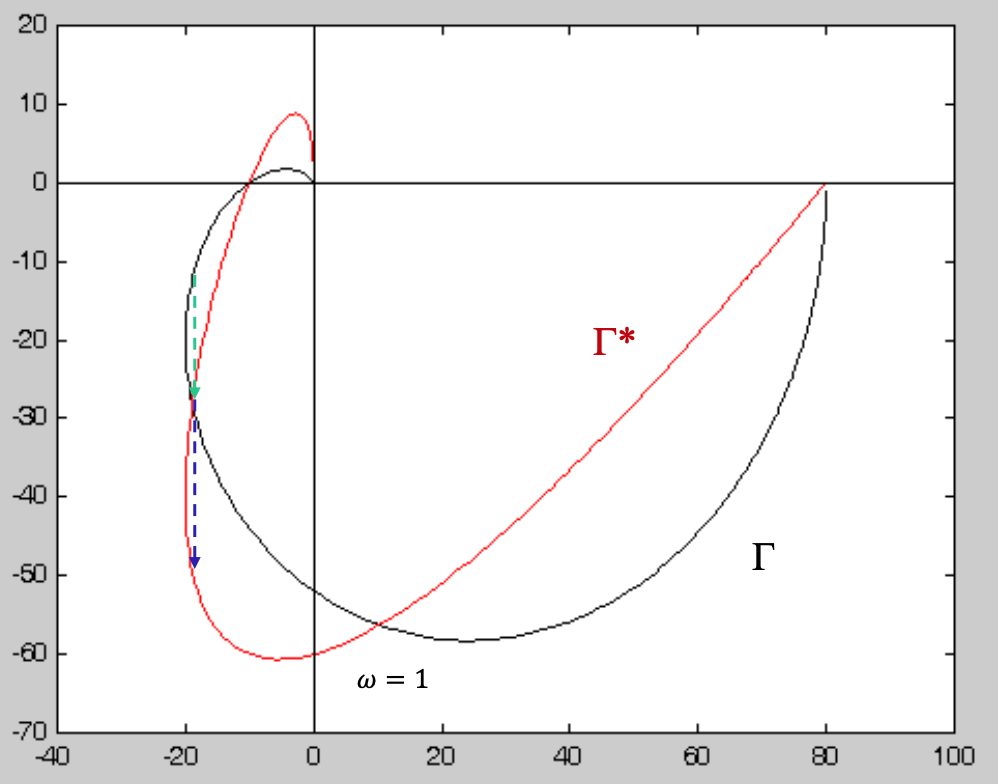
\includegraphics[scale=0.4]{immagini/ex1}
	\caption{Comparison between Popov plot and polar plot of G(s)}
	\label{fig:ex5}
\end{figure}
We know want to identify on the plot $K_N$ and $K_P$.
\begin{figure}[H]
	\centering
	\begin{subfigure}[b]{0.3\textwidth}
		\centering
		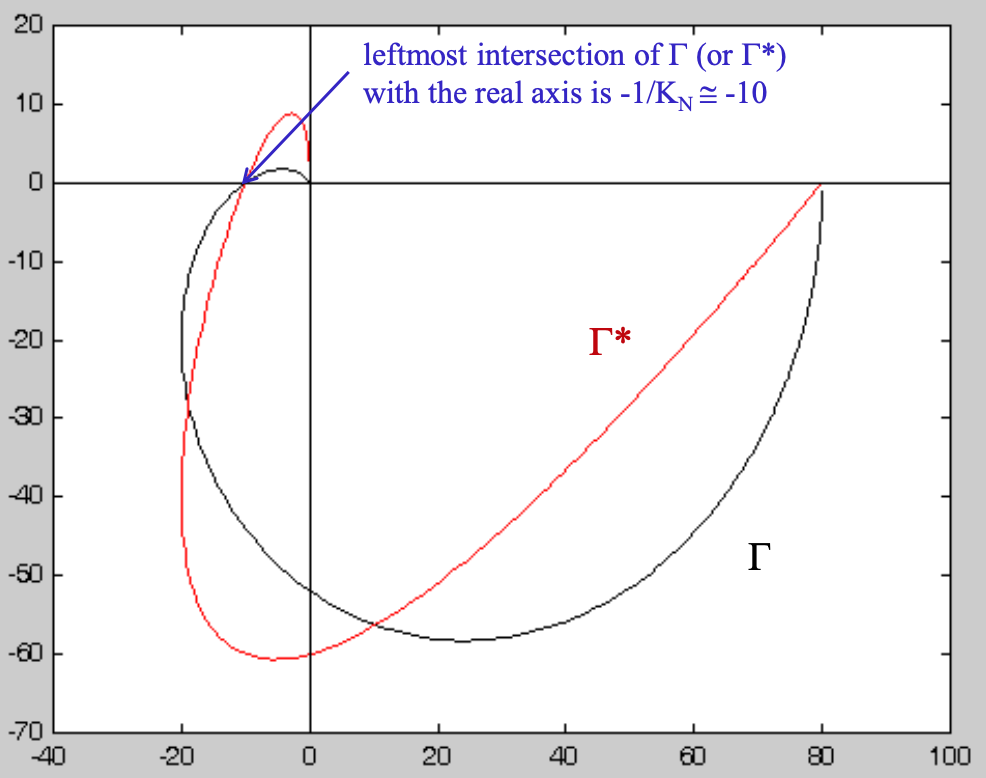
\includegraphics[scale=0.25]{immagini/ex2}
		\caption{$K_N$}
		\label{fig:kn}
	\end{subfigure}
	\hfill
	\begin{subfigure}[b]{0.3\textwidth}
		\centering
		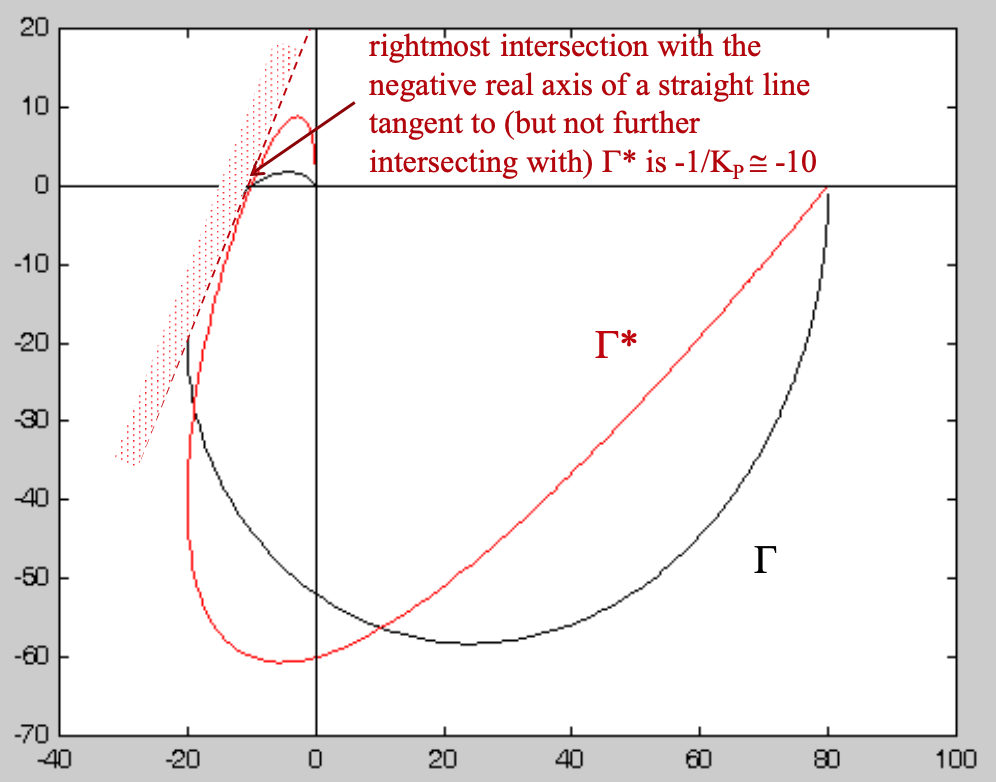
\includegraphics[scale=0.25]{immagini/ex3}
		\caption{$K_P$}
		\label{fig:kp}
	\end{subfigure}
	\hfill
	\label{fig:esempio1}
\end{figure}
In this example $K_P=K_N\cong 0.1$ and, hence, S is absolutely stable in the sector [0,h], for any $h \in [0,0.1)$ and $S_L$ is asymptotically stable for any $h \in [0,0.1)$. $\Longrightarrow$ \textbf{Aizerman conjecture is satisfied}.

\paragraph{Example} Now we will do the same procedure but with a different general transfer function with 3 zeros and 4 poles.\[G(s)=\frac{\mu(1+sT_1)(1+sT_2)^2}{(1+sT_3)^2(1+sT_4)(1+sT_5)}\]
\begin{figure}[H]
	\centering
	\begin{subfigure}[b]{0.3\textwidth}
		\centering
		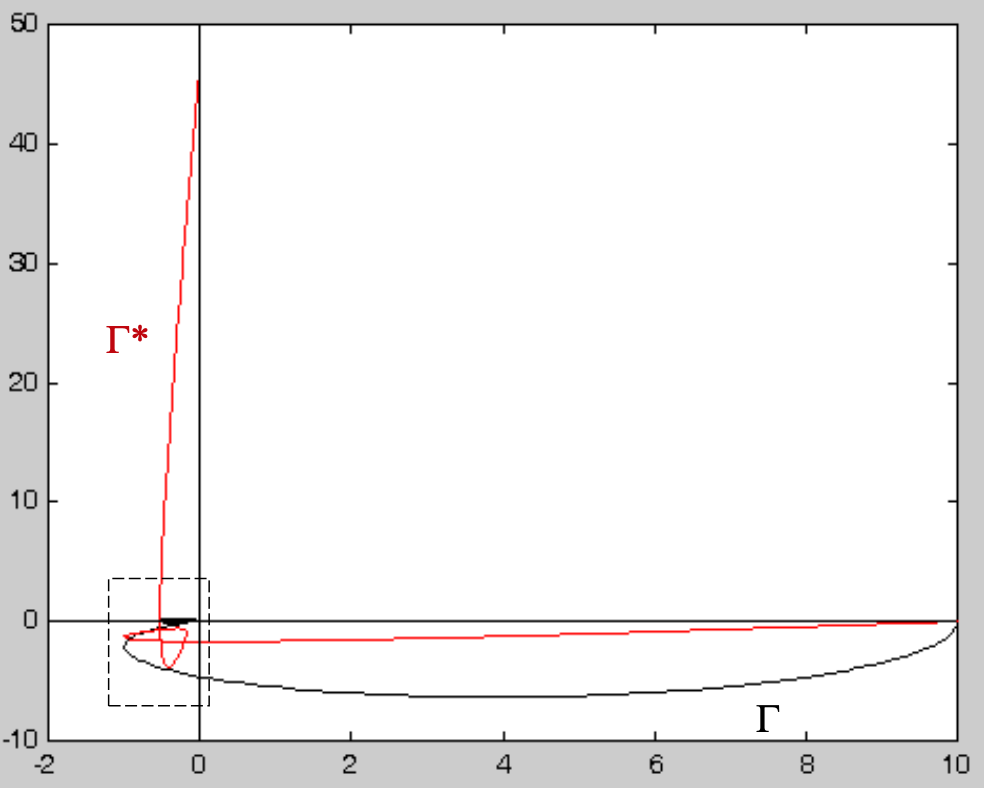
\includegraphics[scale=0.25]{immagini/ex4}
		\caption{$K_P<K_N$ transfer function}
		\label{fig:plopov}
	\end{subfigure}
	\hfill
	\begin{subfigure}[b]{0.3\textwidth}
		\centering
		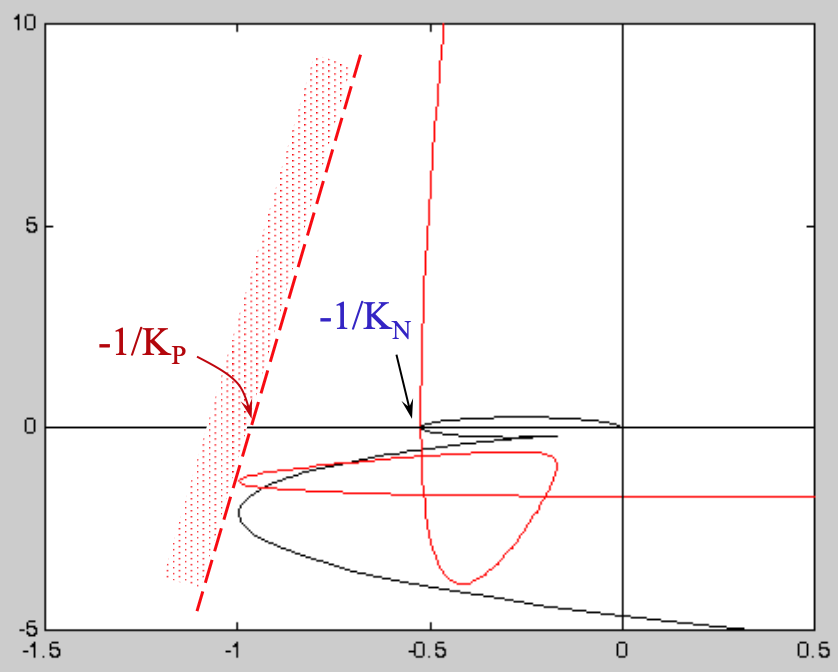
\includegraphics[scale=0.3]{immagini/ex5}
		\caption{$K_N$ and $K_P$ identification}
		\label{fig:kp&kn}
	\end{subfigure}
	\hfill
	\label{fig:esempio2}
\end{figure}
In this example $K_P\cong1.1<K_N\cong1.8$, and, hence, S is absolutely stable in the sector [0,h], for any $h\in[ 0,1.1)$ while $S_L$ is asymptotically stable for any $h\in[0,1.8)$. So, is Aizerman conjecture satisfied? $\Rightarrow$ Maybe ...
\section{Circle criterion}
In this section we will treat the second sufficient condition for absolute condition, the circle criterion, and how is related to the Popov criterion and why can be seen as a corollary of the latter.\\
Since the Popov criterion holds only for nonlinear sector of the shape $[0,k]$ we need to extend the nonlinearity in the sector $[k_1,k_2]$. The trick is to transform the system with nonlinearity in  $[k_1,k_2]$  in another equivalent system but with a sector nonlinearity as the previously aimed $[0,k]$.
\begin{figure}[H]
	\centering
	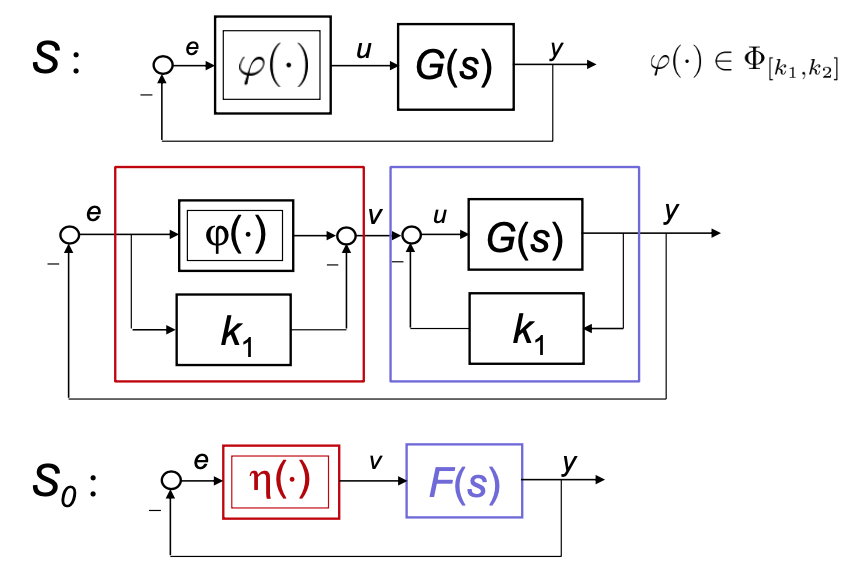
\includegraphics[scale=0.5]{immagini/extensions}
	\caption{Extension to nonlinearity in sector $[k_1,k_2]$}
	\label{fig:extensions}
\end{figure}
\[
\left.
\begin{aligned}
	& \eta(e)=\phi(e)-k_1e, e\in Re	\\
	& k_1e\le \phi(e)\le k_2e,e \in \Re
\end{aligned}
\right\rbrace
\to \eta(\cdot)\in \Phi_{[0,k_2-k_1]}
\]while $F(s)=\frac{G(s)}{1+k_1G(s)}$.\\
From the equivalence between the two systems we have that system S is absolutely stable in the sector $[k_1,k_2]$ if and only if the system $S_0$ is absolutely stable in sector [0,k] with $k=k_2-k_1$.
\begin{note}
	The circle criterion is a restriction of Popov criterion because it requires q=0.
\end{note}
So if q=0, then, we have to check the following conditions:
\begin{enumerate}
	\item F(s) is the transfer function of an asymptotically stable system;
	\item $\Re[F(j\omega)]>-\frac{1}{k}, \forall \omega \ge0$ with $k=k_2-K_1$
\end{enumerate}
\paragraph{Condition 1} G(s) has to satisfy the necessary condition for the absolute stability of S in the sector $[k_1,k_2]$, that is the Nyquist plot of G(s) has to encircle anticlockwise $I(k_1,k_2)$, and hence the point $-\frac{1}{k}$, as many times as the number of poles of G(s) with positive real part. This leads to the result that F(s) is the transfer function of an asymptotically stable system by Nyquist criterion.
\paragraph{Condition 2} We shall rephrase the condition $\Re[F(j\omega)]>-\frac{1}{k}, \forall \omega \ge0$ in an suitable one on the polar plot of $G(j\omega)$.\\
We can map the polar plot of G(s) in function of F(s): $G(s)=F(s)(1+k_1G(s))\to G(s)(1-k_1F(s))=F(s)\to G(s)=\frac{F(s)}{1-k_1F(s)}$. So mapping every point s of F(s) through the transformation $\tilde{s}=\frac{s}{1-k_1s}$ we can draw the polar plot of G(s). And of course also the boundary region has to be transformed and the result will be the circle of the circle criterion that should not be intersected by the polar plot.
\begin{figure}[H]
	\centering
	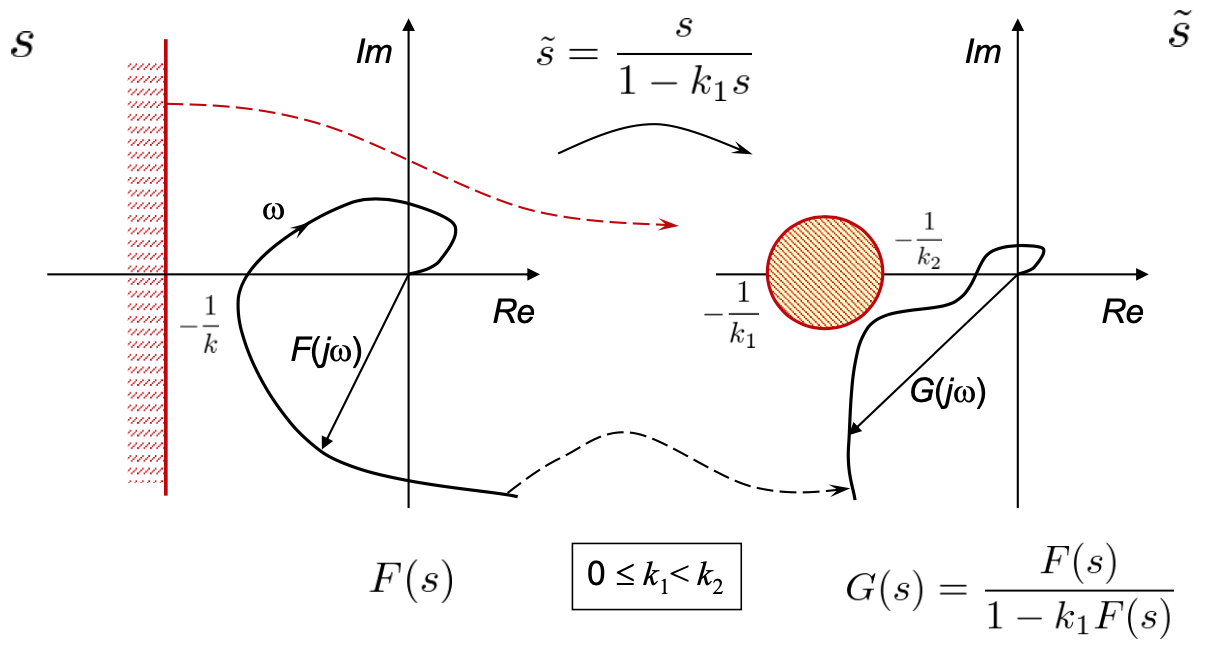
\includegraphics[scale=0.4]{immagini/cond2}
	\caption{Rephrasing of the second condition in a suitable one the polar plot of $G(j\omega)$}
	\label{fig:cond2}
\end{figure}
\begin{note}
	It's not surprising that the left-hand side of the  line is mapped in the inside of the circle because if you take the intersection of the circle with the real axis we get an interval $I(k_1,k_2)$ of the Nyquist criterion, which is a necessary condition to be satisfied by $G(j\omega)$. Since Nyquist criterion is a necessary condition, the plot of $G(j\omega)$ should encircles the interval a number of times equals to the number of pole of $G(j\omega)$ with positive real part. 
\end{note}
Finally we can state a theorem.
\begin{thm}[sufficient condition for the absolute stability of S in the sector \textcolor{red}{$[k_1,k_2]$}, Circle criterion]
	System S is absolutely stable in the sector $[k_1,k_2]$, if the Nyquist plot of G(s) encircles (anti-clockwise) the circle $O(k_1, k_2)$ as many times as the number of poles of G(s) with positive real part.
\end{thm}
\begin{note}
	Since the Circle criterion is a corollary of Popov criterion, if the first fails we can go back to Popov and try with a $q\neq 0$.
\end{note}
\begin{figure}[H]
	\centering
	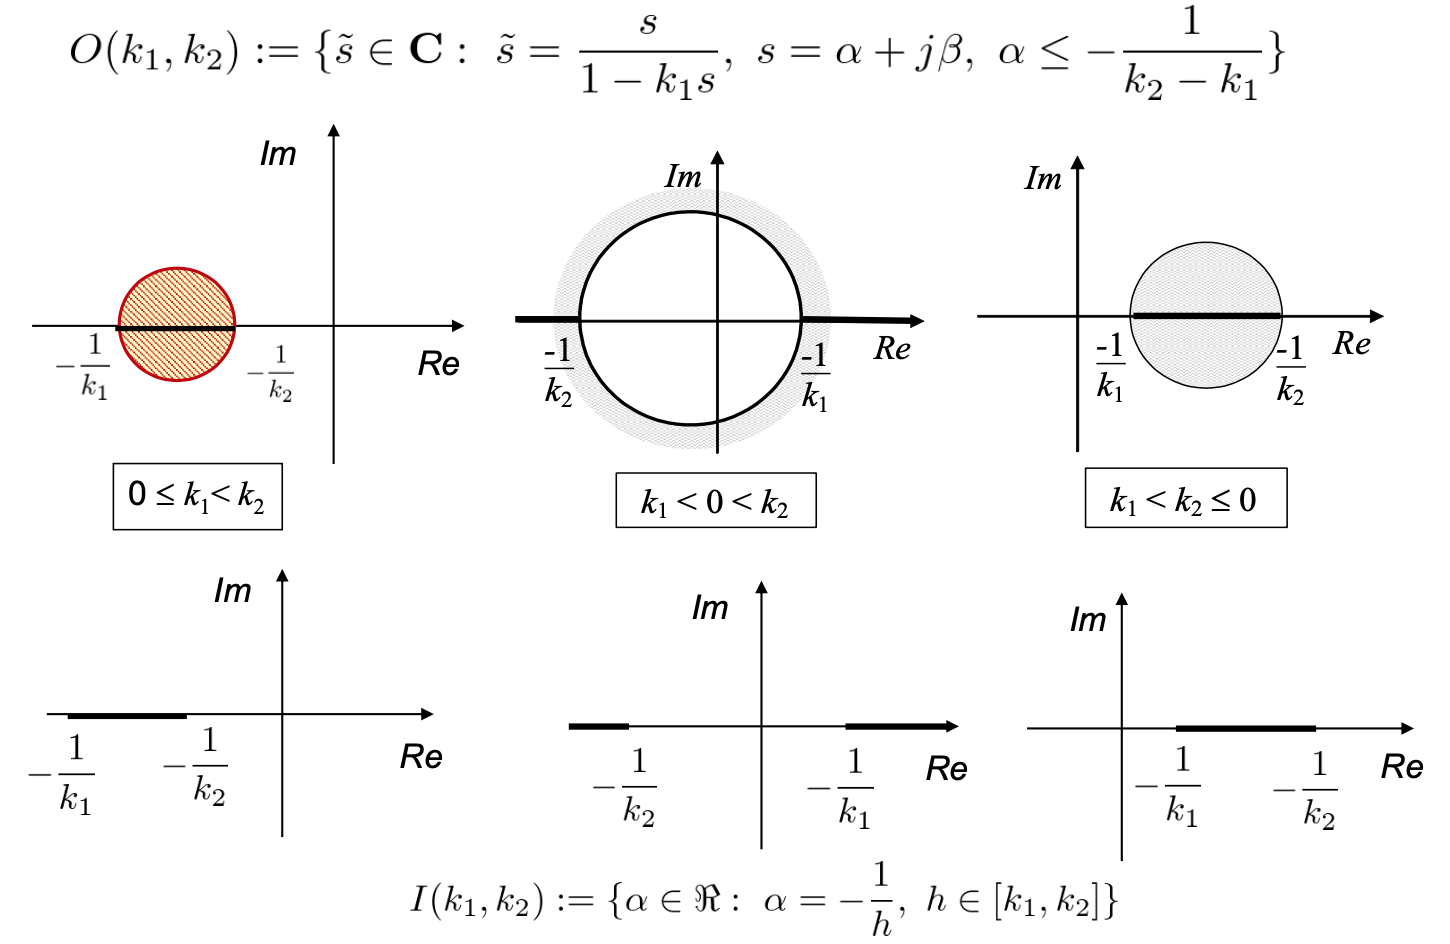
\includegraphics[scale=0.4]{immagini/circpopv}
	\caption{Relation between segments and circle in Circle and Nyquist criterion}
	\label{fig:circpopv}
\end{figure}
\section{Time varying Lur'e systems}
In this section we will analyze again the Lur'e system but this time the nonlinearity is also time varying.\begin{figure}[H]
	\centering
	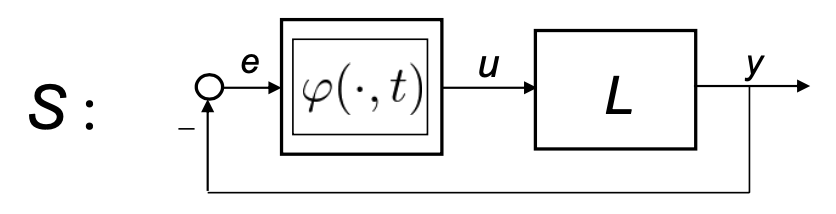
\includegraphics[scale=0.4]{immagini/tvarlur}
	\caption{Time varying non linearity in  Lur'e system}
	\label{fig:tvarlur}
\end{figure}
Given the assumption of reachability of the couple (A,B) and observability of the couple (A,C) the non linear part is defined as follows:
\[
N \colon u(t)=\phi(e(t)), \forall e 
\]
While the linear part is simply:
\[
L:  \begin{cases}
	\dot{x}=Ax+Bu \\ y=Cx
\end{cases}
\] 
\\As before, The $\phi$ function is ment to be continuous and to belong to a \textbf{sector nonlinearity}.
\begin{figure}[H]
	\centering
	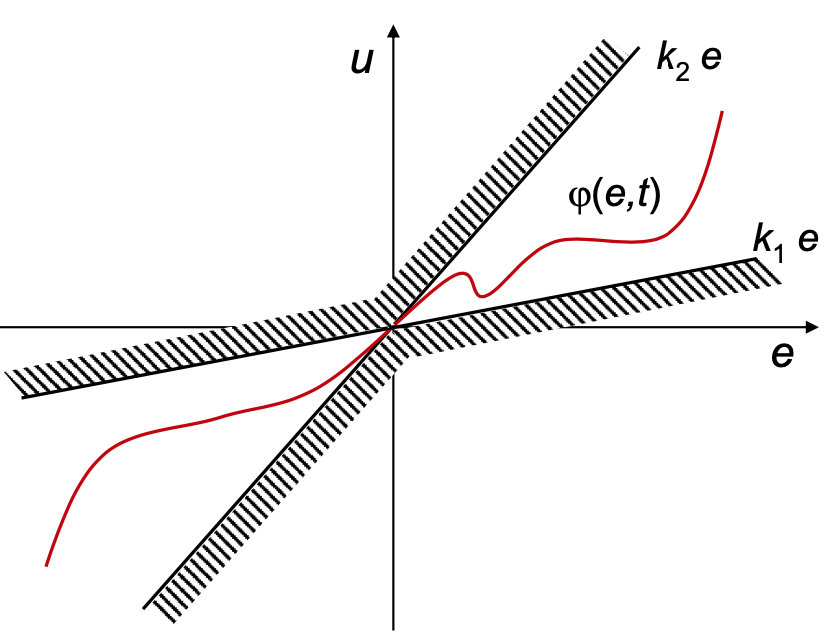
\includegraphics[scale=0.4]{immagini/tvarsec}
	\caption{Nonlinearity for a given $\bar{t}$, the sector remains the same, the curve change.}
	\label{fig:tvarsec}
\end{figure}
The sector is plotted in the e-u space taking e as an input and u as the output and it's defined by two lines of slope $k_1$and $k_2$. The sector of nonlinearity is the sector that contains all the $\phi$ funcitons which satisfy the following condition:
\[
\phi(\cdot,t) \in \Phi_{[k_1,k_2]}=\left\{\phi(\cdot)\colon k_1e^2\le\phi(e)e\le k_2e^2, \forall e \in \Re  \right\} \forall t \in \Re.
\]
Since the sector enforce the function to pass from 0 in any case and: $f(x(t),t)\colon=Ax(t)+B\phi(-Cx(t),t)$ if $\phi(0,\cdot)\to 0$ also $f(0,\cdot)\to 0$ and so $\bar{x}=0$ is an equilibrium for S, for any section nonlinearity $\phi(\cdot,t) \in \Phi_{\left[k_1,k_2\right]}$.

\subsubsection{Absolute stability in the sector $[k_1,k_2]$}
\begin{defn}
	System \textcolor{red}{S} is \textcolor{red}{absolutely stable in the sector $[k_1,k_2]$} if x=0 is a globally \textbf{uniformly} asymptotically stable (GUAS) equilibrium for all nonlinearities in the given sector.
\end{defn}
But now we have to formally explain what is meant with the notion of "uniform" stability.
\subsection{Uniform stability notions}
Given a dynamic system:
\[\dot{x}(t)=f(x(t),t)\] suppose that $f(o,\cdot)=0$. The equilibrium x=0 is:
\begin{itemize}
	\item stable if \[\forall\epsilon>0 \exists \gamma(\epsilon,t_0)>0\colon\|x(t_0)\|>\gamma\to\|x(t)\|<\epsilon,\forall t\ge t_0\]
	\item asymptotically stable if it is stable and \[\exists c(t_0)>0\colon \lim_{t\rightarrow \infty}x(t)=0,\forall\|x(t_0)\|)<c(t_0)	\]
	\item uniformly stable if \[\forall\epsilon>0 \exists \gamma(\epsilon)>0\colon\|x(t_0)\|>\gamma\to\|x(t)\|<\epsilon,\forall t\ge t_0\]
	\item uniformly asymptotically stable if it is uniformly stable and \[ \exists c >0\colon \lim_{t\rightarrow\infty}x(t)=0,\forall \|x(t_0)\|<c\] with convergence to zero that is uniform in $t_0$, i.e \[\forall\epsilon>0\exists T(\epsilon)>0\colon\|x(t)\|<\epsilon\forall t\ge t_0+T(\epsilon),\forall \|x(t_0)\|<c\]
	\item globally uniformly asymptotically stable if it is uniformly stable and \[\forall \epsilon >0 \text{ and } c>0 \exists T(\epsilon,c)> 0\colon\|x(t)\|<\epsilon, \forall t \ge t_0+T(\epsilon,c), \forall\|x(t_0)\|<c\]
\end{itemize}
\subsection{Lyapunov theorem for time varying system} \label{LYAptv}
Let's recall Lyapunov stability theorem for time varying system of the form:\[\dot{x}(t)=f(x(t),t)	\]
Let x=0 be an equilibrium\\If $V\colon [0,\infty]\times 	Re^n\to\Re$ is a $C^1$ function such that:\[W_1(x)\ge V(t,x) \ge W_2(x)\]\[\frac{\delta V}{\delta t}+\frac{\delta V}{\delta x}f(x,t)\le-W_3\] where $W_1(x), W_2(x), W_3(x)$ are continuous and positive definite funcitons, then, x=0 is uniformly asymptotically stable.\\Furthermore, if $W_1(x)$ is radially unbounded, then x=0 is \textbf{globally} uniformly asymptotically stable.\\Consider\[V(t,x)=x'Px,P=P'>0\] as candidate Lyapunov function. Then, one only needs to show that \[\dot{V}(t,x)=f(x,t)'Px+x'Pf(x,t)\le-W_3(x),\forall t\ge 0,\forall x \in \Re^n\] with $W_3(x)$ positive definite.
\begin{proof}
	\[W_1(x)=\lambda_{min(P)}\|x\|^2\le x'Px\le\lambda_{max}(P)\|x\|^2=W_2(x)\] $W_2(x), W_3(x)$ positive definite and $W_1(x)$ radially unbounded
\end{proof}
With this preliminary consideration we are now able to find a sufficient condition for the absolute stability.
\subsection{Necessary condition}
\begin{thm}[Necessary condition for absolute stability of a time invariant Lur'e system]
	If S is absolutely stable in the sector $[k_1, k_2]$, then the Nyquist plot of G(s) encircles (anti-clockwise) $I(k_1,k_2)$ as many times as the number of poles of G(s) with positive real part.
	In particular, if $0\in[k_1, k_2]$, then system L with transfer function G(s) is asymptotically stable.
\end{thm}
\begin{note}
	This theorem is exactly the same as for time invariant Lur'e systems because it is a robust version of Nyquist theorem and we can see the time invariant system as a particular case of the more general time varying. So if it holds for a particularity has to be necessary also for the general case.
\end{note}
\subsection{Popov criterion}
We are not proving it but Popov criterion also holds for time varying case but \textbf{only with q=0}, which is the main difference between time varying and invariant Lur'e systems.
\begin{thm}[sufficient condition for the absolute stability of S in sector \textcolor{red}{[0,k]}, Popov criterion, 1962] 
	System S is absolutely stable in sector [0,k] if system L is asymptotically stable (necessary condition), and if Popov condition is satisfied with q=0.
	\[
	\Re\left[G(j\omega)\right] > -\frac{1}{k}, \forall \omega \ge 0
	\]
\end{thm} And not surprisingly since Popov criterion holds for q=0 we can derive the corollary which is Circle criterion.
\subsection{Circle criterion}
\begin{thm}[sufficient condition for the absolute stability of S in the sector \textcolor{red}{$[k_1,k_2]$}, Circle criterion]
	System S is absolutely stable in the sector $[k_1,k_2]$, if the Nyquist plot of G(s) encircles (anti-clockwise) the circle $O(k_1, k_2)$ as many times as the number of poles of G(s) with positive real part.
\end{thm}
Circle criterion (as we can see the statement it has the same formulation), holds true also for time varying systems but absolute stability has a different meaning. Here we need global uniform asymptotic stability for the zero equilibrium. 
\subsection{Necessary and sufficient condition}
\begin{figure}[H]
	\centering
	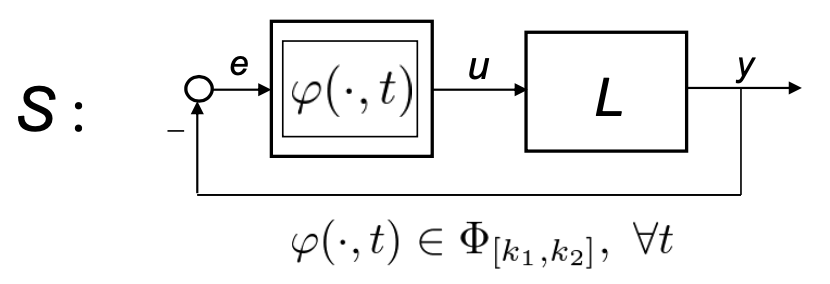
\includegraphics[scale=0.4]{immagini/tvls}
	\label{fig:tvls}
\end{figure}
This time, similar as we did in Section \ref{S_L}, we substitute the nonlinear block with a constant parameter but, this time, time varying which give us more flexibility.
\begin{figure}[H]
	\centering
	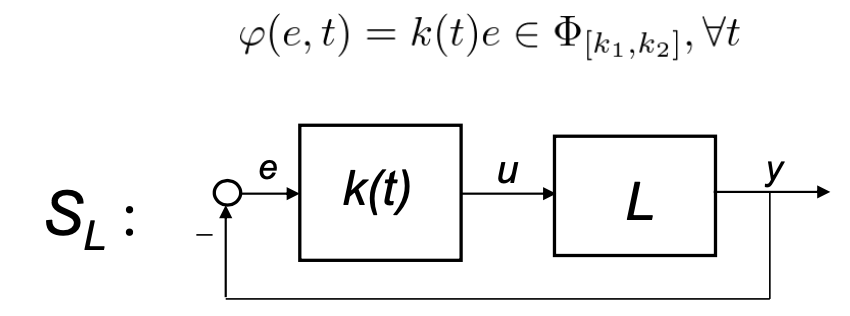
\includegraphics[scale=0.4]{immagini/tvlsl}
	\label{fig:tvlsl}
\end{figure}
So if system $S$ is absolutely stable also $S_L$ is absolutely stable because we have restricted $\phi$. In this case, since the system is linear the stability it's not only absolute but also global, uniform and asymptotical. So this would entail that:\\
S absolute stable in $[K_1,k_2]$ $\leftrightarrow$ $S_L$ is globally uniformly asymptotically stable $\forall k(\cdot)\colon k(t) \in [k_1,k_2], \forall t$.\\But why also the right-to-left implication holds true? We will show in  the following figure.
\begin{figure}[H]
	\centering
	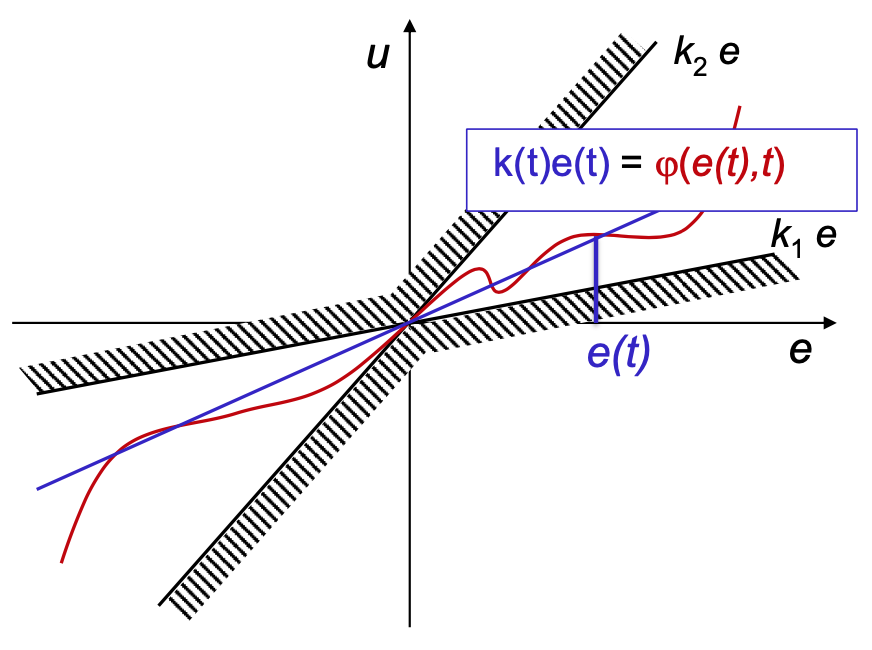
\includegraphics[scale=0.4]{immagini/tvsec}
	\label{fig:tvsec}
\end{figure}
Just thing that at every time instant we have a $\phi$ function (red curve). At every time t we have a certain value of e(t) where we are going to evaluate our $\phi$ function. The line linking the point $\phi(e(t,t))$ to the origin has a slope equal to $k(t)$. So in that point $k(t)e(t)=\phi(e(t,t))$. So actually at every time t and for every e we can find a line with k(t) slope such that the previous equality holds. And this is why the necessary condition is also sufficient.
\begin{thm}[necessary and sufficient condition]
	System S is absolutely stable in the $[k_1, k_2]$ sector \textbf{if and only if} the linear system $S_L$ is globally uniformly asymptotically stable $\forall k(\cdot)\colon k(t) \in [k_1,k_2], \forall t$
\end{thm}
\begin{note}
	Aizerman conjecture is satisfied because when we switch to the linear case we preserve time variability but... it is generally not easy to assess the stability of linear time-varying systems.
\end{note}
\subsection{Global uniform asymptotic stability of $S_L$}
Now what we want to do is proving the global asymptotic stability of the linear system associated to the original system S. In order to do so we will continue the preliminaries concept shown in Section \ref{LYAptv}.
\begin{figure}[H]
	\centering
	\includegraphics[scale=0.4]{immagini/slproof}
	\label{fig:slproof}
\end{figure}
The first thing we can notice is that this system is like a switching system but this time the dynamic switches among a continuum of  system with linear dynamic. Let's introduce some notation.
\[S_L\colon \begin{cases}
	\dot{x}(t)=Ax(t)-Bk(t)Cx(t)=(A-k(t)BC)x(t)\\
	y(t)=Cx(t)
\end{cases}
\]
\[S_L(k)\colon \begin{cases}
	\dot{x}(t)=A_{k(t)x(t)}\\
	y(t)=Cx(t)
\end{cases}
\]
where $A_{k(t)}\colon=A-k(t)BC$ and $k(t) \in [k_1,k_2],\forall t$ \\
Ans, of course, for every value of k we take the matrix A should be Hurwitz. But this is only necessary because as we saw in Section \ref{introstab} and in Figure \ref{fig:12stable} for certain switching sequence the process can loose stability.
\paragraph{Recall on Lyapunov theorem}
Let's recall Lyapunov stability theorem for time varying system of the form:\[\dot{x}(t)=f(x(t),t)	\]
Let x=0 be an equilibrium\\If $V\colon [0,\infty]\times 	Re^n\to\Re$ is a $C^1$ function such that:\[W_1(x)\ge V(t,x) \ge W_2(x)\]\[\frac{\delta V}{\delta t}+\frac{\delta V}{\delta x}f(x,t)\le-W_3\] where $W_1(x), W_2(x), W_3(x)$ are continuous and positive definite funcitons, then, x=0 is uniformly asymptotically stable.\\Furthermore, if $W_1(x)$ is radially unbounded, then x=0 is \textbf{globally} uniformly asymptotically stable.\\Consider\[\boxed{V(t,x)=x'Px,P=P'>0}\] as candidate Lyapunov function. Then, one only needs to show that \[\dot{V}(t,x)=f(x,t)'Px+x'Pf(x,t)\le-W_3(x),\forall t\ge 0,\forall x \in \Re^n\] with $W_3(x)$ positive definite.
This time the quadratic Lyapunov function must be global and common for all the possible dynamics of the switched system.
\begin{prop}[Sufficient condition]
	System $S_L$ is globally uniformly asymptotically stable if there exists $P=P'>0$ such that
	\[
	\left.
	\begin{aligned}
		& A_{k_2}'P+PA_{k_2}<0\\
		& A_{k_1}'P+PA_{k_1}<0
	\end{aligned}
	\right\rbrace
	\qquad S_L(k_1)\text{ and }S_L(k_2) \text{admit the same quadratic Lyapunov function } x'Px
	\]
\end{prop}
It's computationally easy to prove this proposition because we just have to solve two LMIs. The trivial part is to prove that is enough to test only $k_1$ and $k_2$ when k indeed can arrange arbitrarily between $k_1$ and $k_2$. The point is to use the previous theorem and show that $V(t,x)=x'Px$ is a global quadratic Lyapunov function.
\begin{proof}
	In order to do that we express the generic dynamic matrix associated to k(t) as a combination according to a coefficient $\alpha(t)$\\
	$A_{k(t)}=\alpha(t)A_{k_2}+(1-\alpha(t))A_{k_1}, \qquad \alpha(t)\in [0,1]$ \\
	with $\alpha(t)=\frac{k(t)-k_1}{k_2-k_1}$
Now the trick is to compute the derivative of our candidate global Lyapunov function along the trajectory of the time invariant system whose dynamic is $A_{k(t)}$ and prove that it is upper bounded from a $W_3(x)$ positive definite
\begin{align*}
	\dot{V}(t,x)&=x'(A_{k(t)}'P+PA_{k(t)})x \\
	&= x'(\alpha(t)A_{k_2}+(1-\alpha(t))A_{k_1})'P+P(\alpha(t)A_{k_2}+(1-\alpha(t))A_{k_1})x\\ &=\alpha(t)x'(A_{k_2}'P+PA_{k_2})x+(1-\alpha(t))x'(A_{k_1}'P+PA_{k_1})x
\end{align*}
Adding $\gamma I$ we are shifting the eigenvalues of this negative definite matrix, but we chose a gamma such that we preserve the definite negativeness. Since we have two matrices we will have two gammas, so we take the smaller one. This condition guarantee that if a multiplication between x' and x ,it is still negative definite.
\[
\exists\gamma>0\colon \begin{cases}
	A_{k_2}'P+PA_{k_2}+\gamma I \le0\\
A_{k_1}'P+PA_{k_1}+\gamma I \le0
\end{cases}\Rightarrow \begin{cases}
x'(A_{k_2}'P+PA_{k_2})x\le -\gamma x'x\\
x'(A_{k_1}'P+PA_{k_1})x\le -\gamma x'x
\end{cases}
\]
So we can replace this two inequality in the expression of the derivative of the Lyapunov function.
\begin{align*}
	\dot{V}(t,x)&=\alpha(t)x'(A_{k_2}'P+PA_{k_2})x+(1-\alpha(t))x'(A_{k_1}'P+PA_{k_1})x\\
	&\le -\alpha(t)\gamma x'Ix-(1-\alpha(t))\gamma x'Ix = -\boxed{\gamma x'x}\longrightarrow W_3(x)
\end{align*}
\end{proof}
\begin{remark}
	Stability is exponential
\[
\left.
\begin{aligned}
	& \dot{V}(x)\le-\gamma \|x\|^2\\
	& V(x)\le \gamma_{max}(P)\|x(t)\|^2\to -\|x\|^2 \le-\frac{V(x)}{\lambda_{max}(P)}	
\end{aligned}
\right\rbrace\qquad	\dot{V}(x)\le -\frac{\gamma}{\lambda_{max}(P)}V(x)
\]
So now we have a \emph{differential inequality} of the form \emph{$f'(x)\le Af(x)$} so the solution is of the form $f(x)=e^{At}f(x_0)$
\[
\dot{V}(x)\le -\frac{\gamma}{\lambda_{max}(P)}V(x)\longrightarrow V(x(t))\le e^{-\frac{\gamma}{\lambda_{max}(P)}}V(x(0))
\]
We also know that $\lambda_{min}(P)\|x(t)\|^2\le V(x)$ which is the lower bound and so, substituiting in the previous equation we get:
\[
\lambda_{min}(P)\|x(t)\|^2\le e^{-\frac{\gamma}{\lambda_{max}(P)}t}\lambda_{max}(P)\|x(0)\|^2
\]
and finally the convergence rate is:
\[
\|x(t)\|\le \sqrt{\frac{\lambda_{max}(P)}{\lambda_{min}(P)}}e^{-\frac{\gamma}{2\lambda_{max}(P)}t}\|x(0)\|.
\]
\end{remark}
%%%%%%Fine Capitolo%%%%%